\documentclass{beamer}
\usepackage[utf8]{inputenc}
\usepackage{caption}
\usepackage{subcaption}

\title{Numerical methods for Extreme Mass Ratio Inspirals of Black Hole Binaries}
\author{Steven Dorsher}
\institute{Louisiana State University}
\date{October 2, 2017}

\begin{document}
\frame{\titlepage}


%\begin{frame}
%  \frametitle{Gravitational Waves}
%  \begin{figure}
%    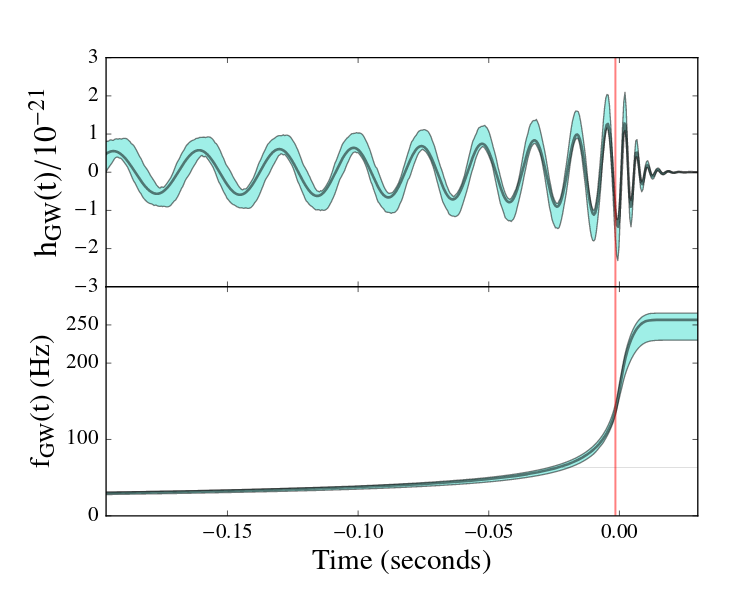
\includegraphics[width=3.0in]{LIGOGRtest.png}
%    \caption{LIGO detection, September 14, 2015. General relativity was tested by comparing inpsiral with merger/ringdown phases.}
%  \end{figure}
%\end{frame}







\begin{frame}
  \frametitle{Toward LISA EMRI templates}
  \begin{itemize}
  \item Generating LISA EMRI templates requires evolving $10^6$ orbits with precision on the order of $\delta P/P\sim 10^{-6}$ {\em Danzmann, Karsten. LISA: A proposal in response to the ESA call for L3 mission concepts (2017)}
  \item For EMRI's, the self-force approximation is used in the limit where the mass ratio is large ($10^4$ to $10^6$)
  \item EMRI's have an orbital evolution timescale that scales as $M/\mu$, and a period that scales as $M$. These two widely different timescales necessitate a different numerical approach than numerical relativity.
  \item Self-force prescribes a perturbative approximation in the mass ratio. 
  \end{itemize}
\end{frame}

%\begin{frame}
%  \frametitle{Self-force in a classical atom}
%  \begin{itemize}
%  \item Consider a classical atom without quantization (not even a Bohr atom)
%  \item The electron orbits the nucleus
%  \item It radiates energy because it is accelerated
%  \item Because it radiates energy, it becomes more tightly bound
%  \item The electron spirals inward due to the interaction of the particle with its own field
%  \item This inspiral is caused by the self-force 
%  \end{itemize}
%\end{frame}

\begin{frame}
  \frametitle{Self-force in general relativity}
  \begin{itemize}
  \item In general relativity, test particles move along geodesics
  \item A compact object is not a test particle
  \item Motion $\rightarrow$ radiation $\rightarrow$ energy and angular momentum loss $\rightarrow$ inspiral
  \item Applies to scalar, electromagnetic, and tensor fields on a gravitational background
  \item Perturbative expansion in powers of the mass ratio
  \end{itemize}
\end{frame}

\begin{frame}
  \frametitle{Goals for the self-force community and this project}
  The long term goal for the field is to generate extremely precise EMRI gravitational wave templates for LISA.

  \begin{itemize}
  \item Scalar rather than tensor waves ($\Psi$ rather than $h_{\mu\nu}$)
  \item Non-rotating black holes: Schwarzschild spacetime
  \end{itemize}

  The state of the art is
  \begin{itemize}
  \item Kerr eccentric inclined geodesics for scalar fields 
  \item Kerr geodesics for gravitational fields with nearly extremal spin
  \item Adiabatic evolution in Schwarzschild or Kerr spacetime in the orbital plane
  \item Scalar unbound orbits in Schwarzschild spacetime
  \item Scalar Schwarzschild self-consistent evolution to low accuracay
  \end{itemize}
  
\end{frame}


\begin{frame}
  \frametitle{Intermediate goals}
  \begin{enumerate}
  \item To port a sample self-force simulation provided by Peter Diener from Fortran to C++ and parallelize it in HPX for the purpose of helping to develop the HPX parallelization system and numerical methods in the self-force field. 
  \item To assess the accuracy of Peter Diener's existing Discontinuous Galerkin eccentric orbit simulation.  
  \end{enumerate}
\end{frame}

\begin{frame}
  \frametitle{A generic wave equation solver}
  Wave equation:
  \begin{equation}
    \Box\Psi=RHS(r,t)
  \end{equation}
  Can be written in state-vector form:
  \begin{equation}
  \frac{\partial u}{\partial t} = A\frac{\partial u}{\partial r} + Bu = RHS(u,t)
  \end{equation}

  Use Discontinuous Galerkin method: truncation error scales as $h^{N+1}$
\end{frame}
  
\begin{frame}
  \frametitle{Flat spacetime evolution}
  \begin{figure}
    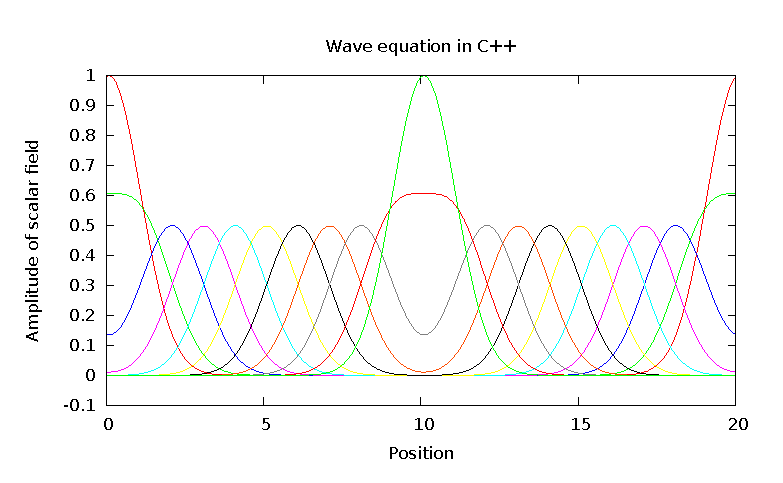
\includegraphics[width=4.0in]{gaussWave}
    \caption{Gaussian initial conditions, flat spacetime}
  \end{figure}
\end{frame}



\begin{frame}
  \frametitle{Flat spacetime error convergence}
  \begin{figure}
    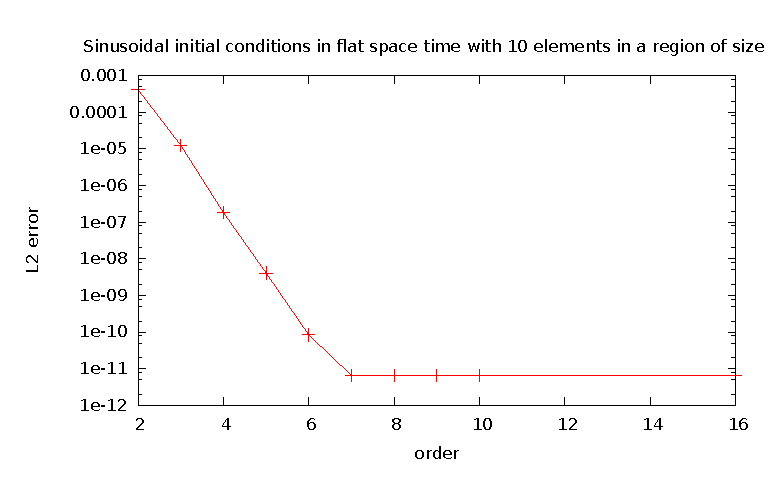
\includegraphics[width=4.0in]{sinL2WTorder}
    \caption{$L_2$ error converges exponentially until it hits roundoff noise with DG order for sinusiodal initial conditions with ten elements of size $h=0.01$.}
  \end{figure}
\end{frame}

\begin{frame}
  \frametitle{Schwarzschild spacetime without a source}
  \begin{itemize}
  \item Wave equation: $\Box\Psi=\frac{1}{\sqrt{-g}}\partial_\mu\left(g^{\mu\nu}(\partial_\nu\Psi)\sqrt{-g}\right)=0$
  \item Multipole moment decomposition to account for angular dependence
  \end{itemize}
\end{frame}
  
\begin{frame}
  \frametitle{Quasinormal mode (QNM) ringing}
  \begin{itemize}
  \item Similar to black hole ringdown phase after a merger
  \item Due to interactions of the scalar field with the background at the peak of the potential
  \item Higher frequencies and faster decay for higher $l$
  \end{itemize}
\end{frame}


\begin{frame}
  \frametitle{Quasinormal modes}
  \begin{figure}
    \centering
    \begin{subfigure}{.45\textwidth}
      \centering
      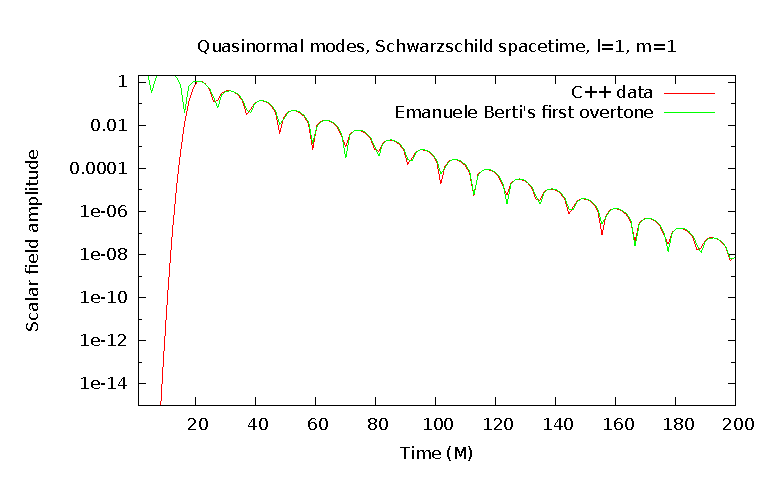
\includegraphics[width=\textwidth]{l1m1qnm}
      \caption{$l=1$}
    \end{subfigure}
    \begin{subfigure}{.45\textwidth}
      \centering
      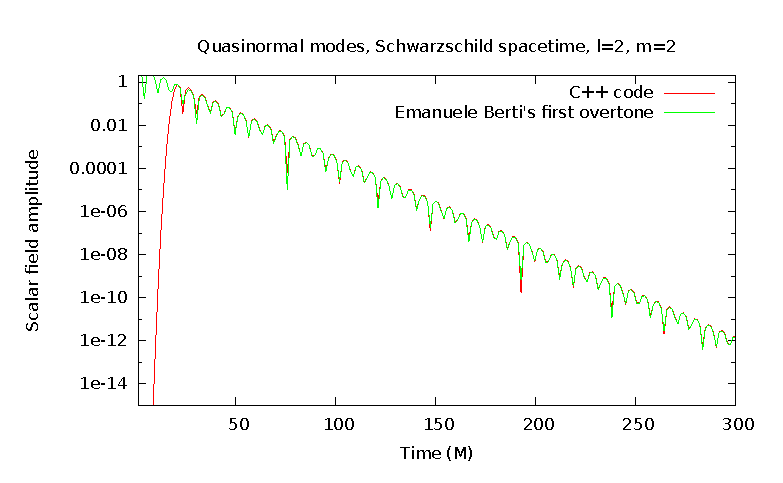
\includegraphics[width=\textwidth]{l2m2qnm}
      \caption{$l=2$}
    \end{subfigure}
  \caption{$l=2$ has a higher frequency and a faster decay rate than $l=1$}
  \end{figure}
\end{frame}

\begin{frame}
  \frametitle{Power law tails}
  \begin{itemize}
  \item Due to scattering off spacetime far from the central black hole
  \item Follow the QNM
  \item Go as $t^{-(2l+3)}$
  \end{itemize}
\end{frame}

\begin{frame}
  \frametitle{Power law tails}
  \begin{figure}
    \centering
    \begin{subfigure}{.45\textwidth}
      \centering
      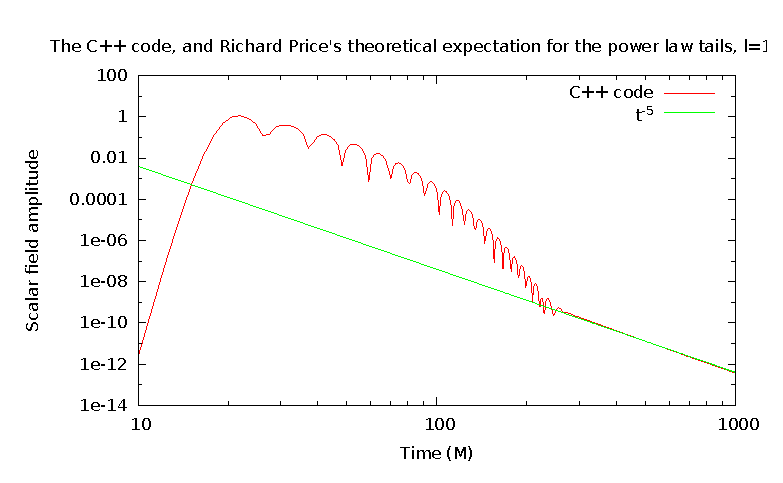
\includegraphics[width=\textwidth]{l1m1tail2}
      \caption{$l=1$}
  \end{subfigure}
    \begin{subfigure}{.45\textwidth}
      \centering
      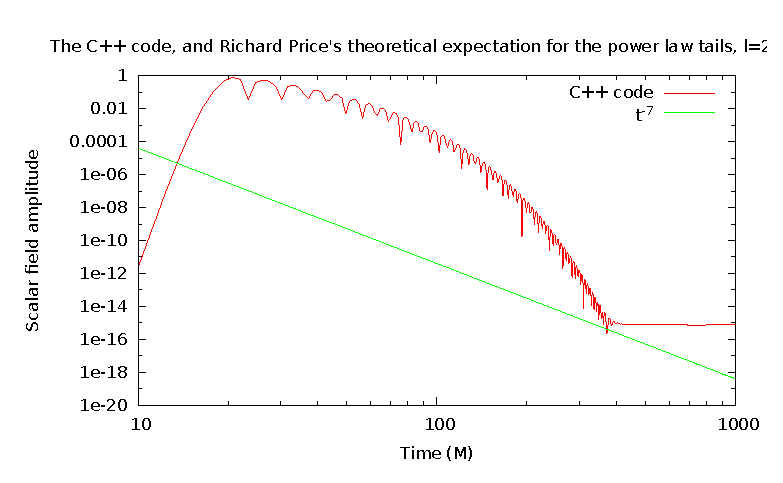
\includegraphics[width=\textwidth]{l2m2tailfail2}
      \caption{$l=2$}
    \end{subfigure}
  \caption{$l=1$ decays as $t^{-5}$ as expected; however, $l=2$ has no power law tail due to truncation error}
  \end{figure}
\end{frame}


\begin{frame}
  \frametitle{A source on a geodesic}
  \begin{itemize}
    \item$\Box\Psi^{ret}=-4\pi q\delta_4(x,z(\tau^\prime))d\tau^\prime$
    \item Detweiler-Whiting singular field: {\em Steven Detweiler, Bernard F. Whiting (2002). Phys. Rev. D 67, 024025}
    \item Source is siingular at location of particle
    \item Regularize field: $\Psi^R=\Psi^{ret}-\Psi^S$
    \item Only know approximation to DW singular field, $\tilde{\Psi}^S$
    \item Limit the effect of the approximation using a world tube window function
  \item $\Box\Psi^R=S_{eff}=\Box\Psi^{ret}-\Box(W\tilde{\Psi}^S)$
  \item HOW effective source: {\em Anna Heffernan, Adrian Ottewill, Barry Wardell (2013). Phys. Rev. D 82 104023}
  \end{itemize}
\end{frame}

\begin{frame}
  \frametitle{Circular orbit roundoff error comparison between languages}
  \begin{figure}
    \centering
    \begin{subfigure}{.45\textwidth}
      \centering
      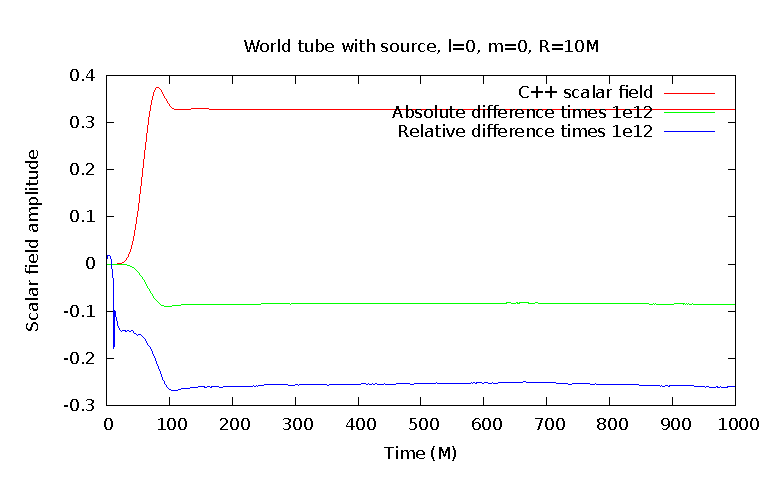
\includegraphics[width=\textwidth]{wtcircl0m0}
      \caption{l=0}
   \end{subfigure}
    \begin{subfigure}{.45\textwidth}
      \centering
      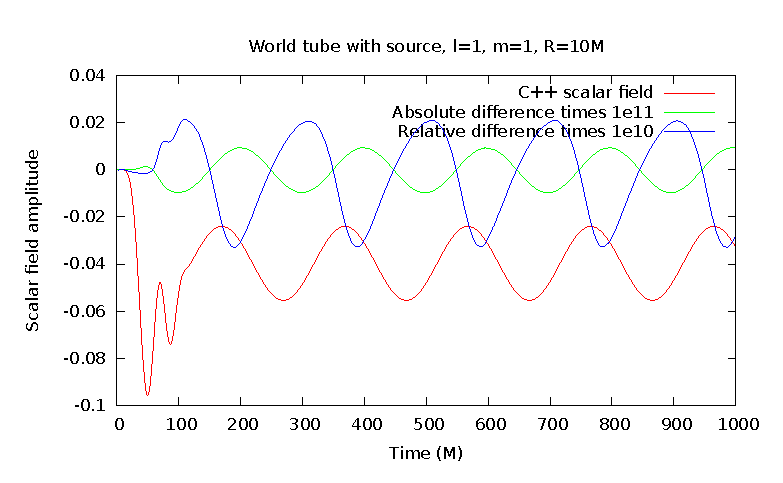
\includegraphics[width=\textwidth]{wtcircl1m1}
      \caption{l=1}
    \end{subfigure}
  \caption{Relative and absolute errors are at the roundoff level-- $10^{-10}$ to $10^{-12}$. Oscillations do not appear in the $l=0$ mode but appear with the orbital period in the $l=1$ mode.}
  \end{figure}
\end{frame}


\begin{frame}
  \frametitle{Eccentric orbits using Peter Diener's simulation}
  \begin{itemize}
  \item $\chi$: radial evolution angle, $\phi$: angular evolution angle $\rightarrow$ precession because they are out of phase
  \item The orbit is held fixed on a geodesic to counteract the self-force generating the scalar waves
  \item $r_{periastron}=\frac{pM}{1+e}$, $r_{apastron}=\frac{pM}{1-e}$
  \item Radial self-force: $F_r=q\partial_r\Psi^R$
  \end{itemize}
\end{frame}

\begin{frame}
  \frametitle{Precession of the eccentric orbit}
  \begin{figure}
    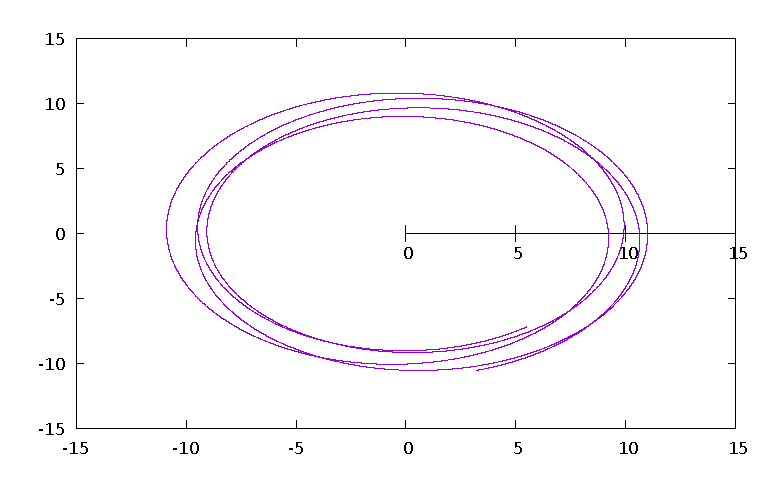
\includegraphics[width=0.9\textwidth]{orbitevolvedg44p99e01}
    \caption{Precession of the eccentric orbit. $p=9.9$, $e=0.0$.}
  \end{figure}
\end{frame}


\begin{frame}
  \frametitle{Evolution of the radial self-force for different initial conditions}
  \begin{figure}
  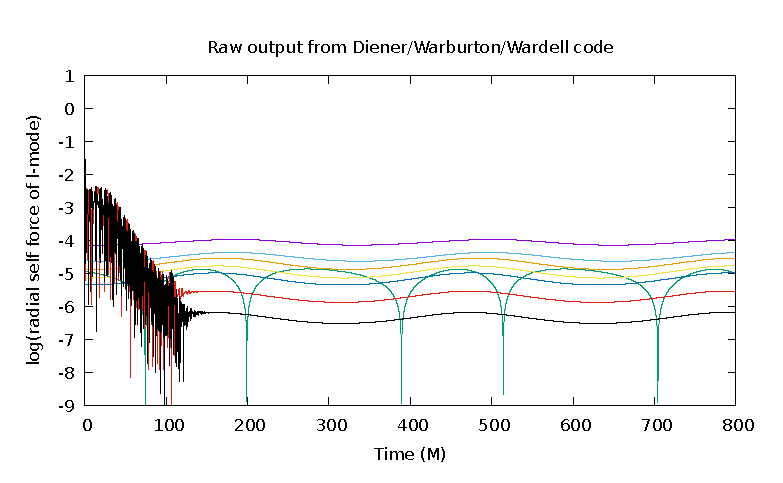
\includegraphics[width=0.9\textwidth]{rawRadialSelForceModes}
  \caption{Low $l$ behavior of the self-force for a given l-mode summed over $m$}
  \end{figure}
\end{frame}



\begin{frame}
  \frametitle{Self-force spherical harmonic components depend on time}
  \begin{figure}
    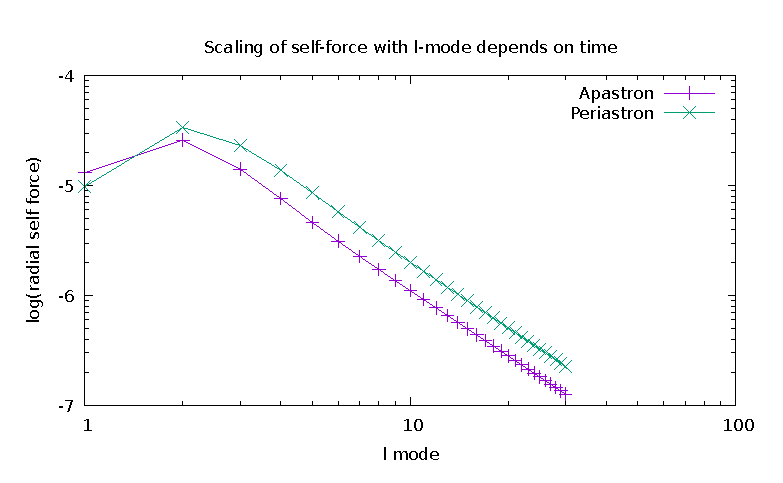
\includegraphics[width=0.9\textwidth]{lmodescalingdependsontime}
    \caption{Periastron has a higher self-force amplitude for nearly every spherical harmonic than apastron.}
  \end{figure}
\end{frame}

\begin{frame}
  \frametitle{The first order Richardson extrapolation}
  \begin{itemize}
  \item Discontinuous Galerkin: ODE solver with truncation errors that scale as $h^{n+1}$
  \item Assume $F_r(n,l)=F_{inf}(l)+c(l)\exp(-\alpha n)$
  \item Obtain extrapolation by solving system of equations for $F_r(n_i,l)$, $i=1,2,3$
   \end{itemize}
\end{frame}

\begin{frame}
  \frametitle{Well-converging data}
  \begin{figure}
  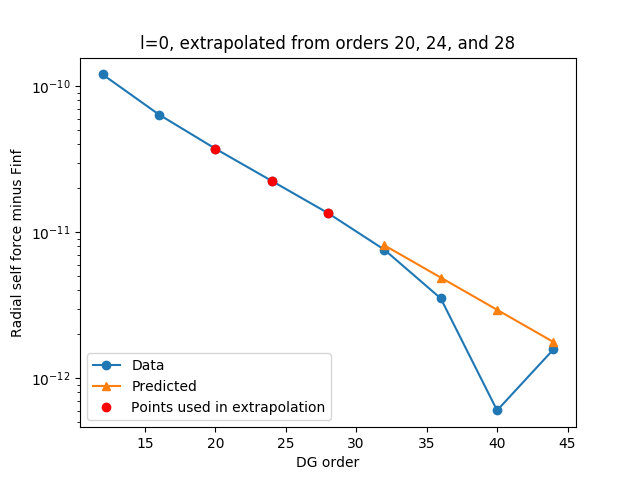
\includegraphics[width=0.9\textwidth]{fittingtechniqet370l0}
  \caption{l=0 at t=370. This data converges very cleanly until it hits roundoff noise at high DG orders.}
  \end{figure}
\end{frame}
  

\begin{frame}
  \frametitle{Error due to neglecting the first order Richardson extrapolation}
  \begin{figure}
    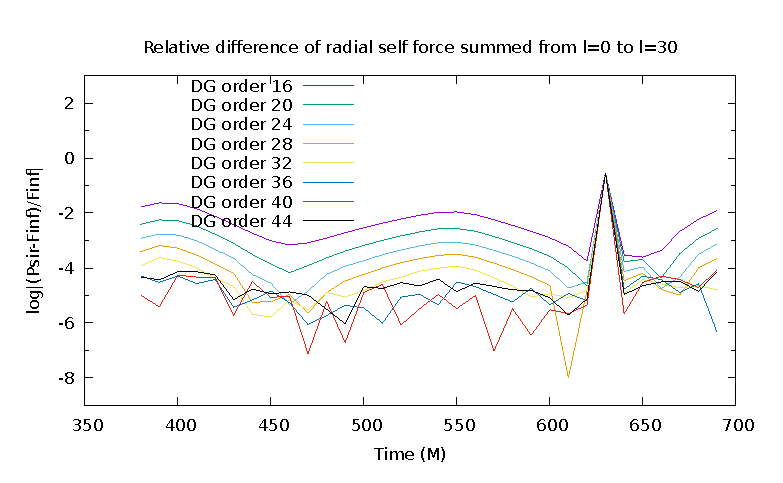
\includegraphics[width=0.9\textwidth]{reldiffpsirvtwfinfdgorders2}
    \caption{Relative error between DG starting orders and $F_{inf}$ vs time. For DG order 36 where roundoff error sets in, the error is about $10^{-4}$.}
  \end{figure}
\end{frame}

\begin{frame}
  \frametitle{The l-mode sum and fit}
  \begin{itemize}
  \item Use spherical harmonic decomposition of $\Psi$ to encode angular information
  \item must sum over $l$ and $m$ at end to obtain self force
  \item Use fit to extend sum to $l=\infty$
  \end{itemize}
  
  \begin{eqnarray}
    F_r(l,t)=&\frac{A(t)}{(2l-1)(21+3)}+\frac{B(t)}{(2l-3)(2l-1)(2l+3)(2l+5)}\nonumber \\
    &+\frac{C(t)}{(2l-5)(2l-3)(2l-1)(2l+3)(2l+5)(2l+7)}+\ldots
  \end{eqnarray}

   {\em Anna Heffernan, Adrian Ottewill, Barry Wardell (2012). Phys. Rev. D 86, 104023}

  \begin{itemize}
  \item Fit from $l_{min}$ to $l_{max}$.
  \item Sum numerically from zero to $l_{max}$ then use fit coefficients to analytically sum to $l=\infty$

  \end{itemize}
\end{frame}


\begin{frame}
  \frametitle{l-mode fit}
  \begin{figure}
    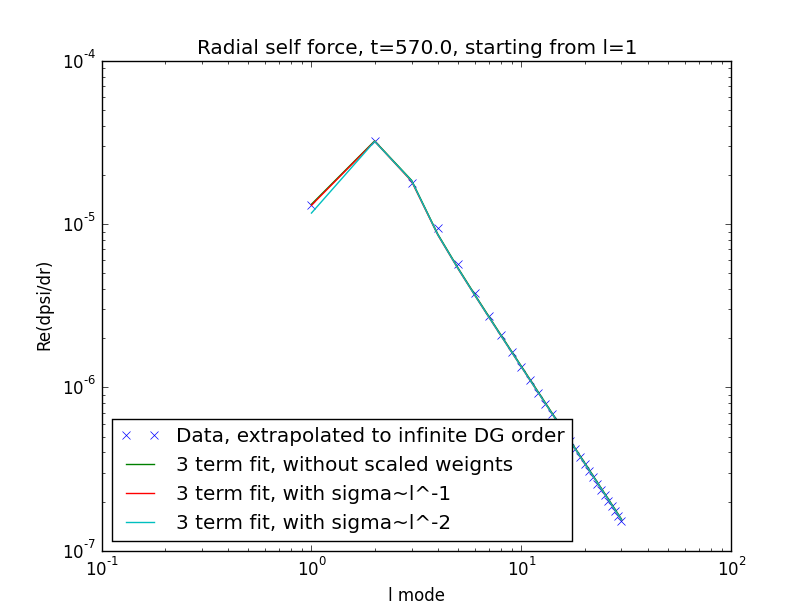
\includegraphics[width=0.9\textwidth]{fiterrscalecorrect3term570l1}
    \caption{l-mode versus $F_{inf}$.}
  \end{figure}
\end{frame}

\begin{frame}
  \frametitle{Residuals to the l-mode fit}
  \begin{figure}
    \centering
    \begin{subfigure}{.45\textwidth}
      \centering
      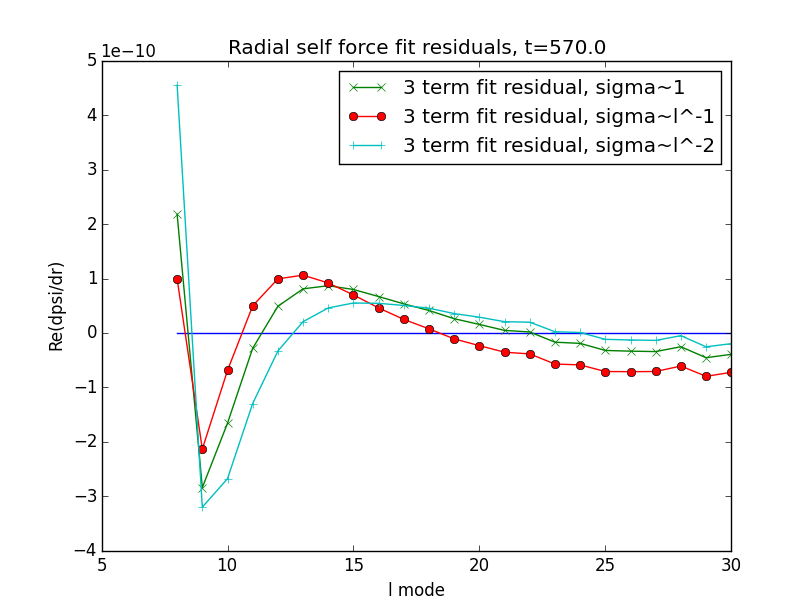
\includegraphics[width=\textwidth]{fitresiduals3terms570l8}
      \caption{$l_{min}=8$}
    \end{subfigure}
    \begin{subfigure}{.45\textwidth}
      \centering
      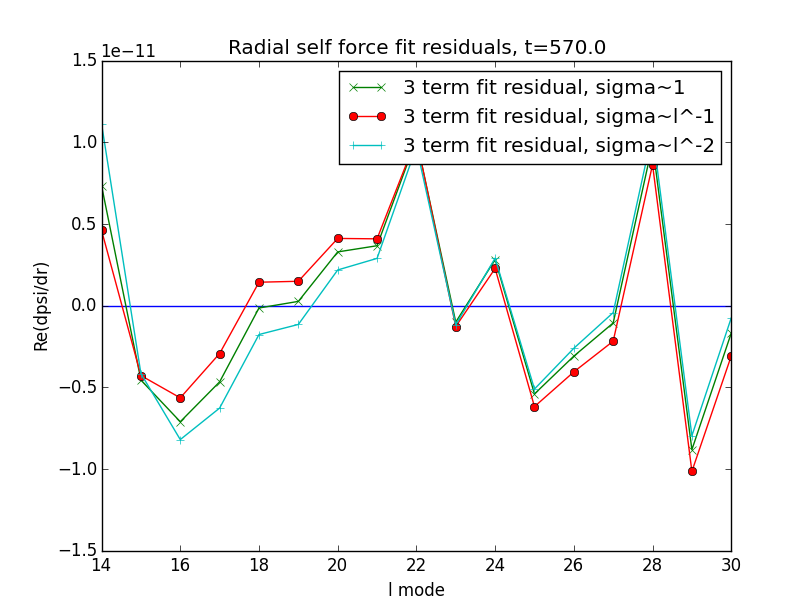
\includegraphics[width=\textwidth]{fitresidulas3terms570l14}
      \caption{$l_{min}=14$}
    \end{subfigure}
  \caption{$l_{min}=14$ is a better fit than $l_{min}=8$ both because it is less systematically biased and because it has an amplitude an order of magnitude smaller. Both fits end at $l_{max}=30$.}
  \end{figure}
\end{frame}

\begin{frame}
  \frametitle{Roundoff noise in $F_{inf}$ at high $l_{max}$}
  \begin{figure}
    \centering
    \begin{subfigure}{.45\textwidth}
      \centering
      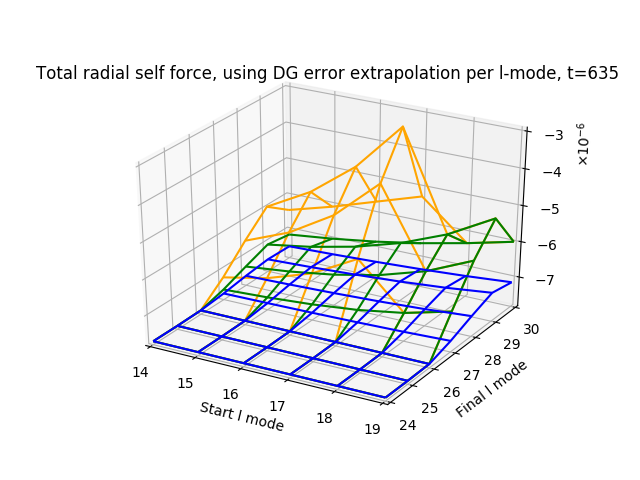
\includegraphics[width=\textwidth]{bestfinflminlmax234terms635fullrange_perihelion}
      \caption{Large range}
    \end{subfigure}
    \begin{subfigure}{.45\textwidth}
      \centering
      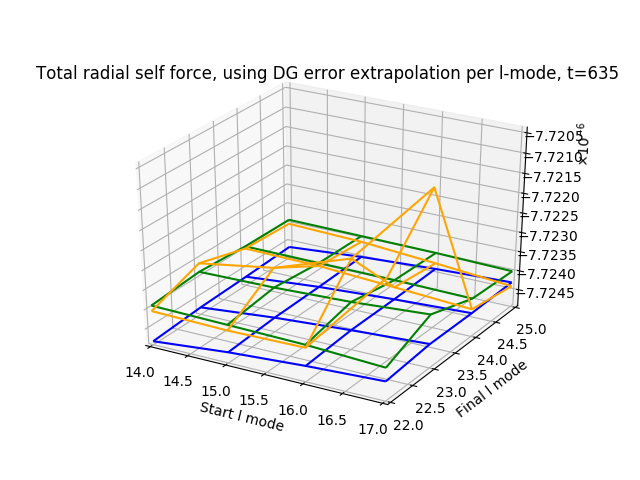
\includegraphics[width=\textwidth]{bestfinflminlmax234termst635smallrange_perihelion}
      \caption{Small range}
    \end{subfigure}
  \caption{$l_{min}=14$ and $l_{max}=25$ appear to be good start and stop values. Roundoff noise is evident at higher l.}
  \end{figure}
\end{frame}


\begin{frame}
  \frametitle{Error due to l-mode selection, number of terms}
  \begin{figure}
    \centering
    \begin{subfigure}{.45\textwidth}
      \centering
      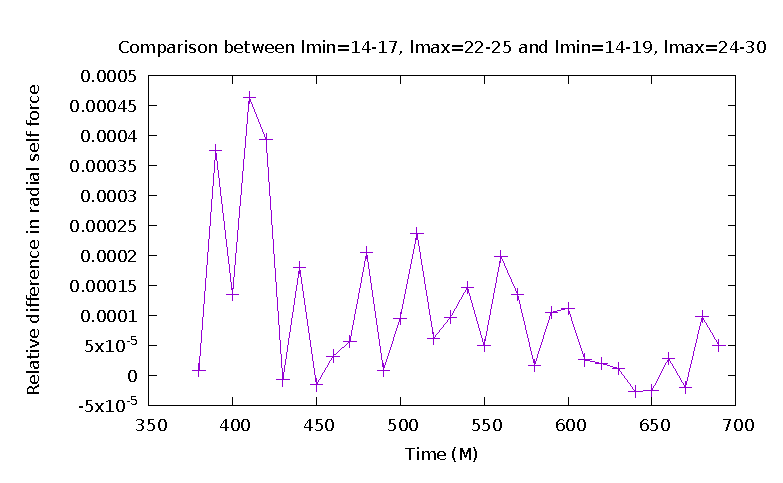
\includegraphics[width=\textwidth]{relErrBigSmallRangeOverTime}
      \caption{large versus small range}
    \end{subfigure}
    \begin{subfigure}{.45\textwidth}
      \centering
      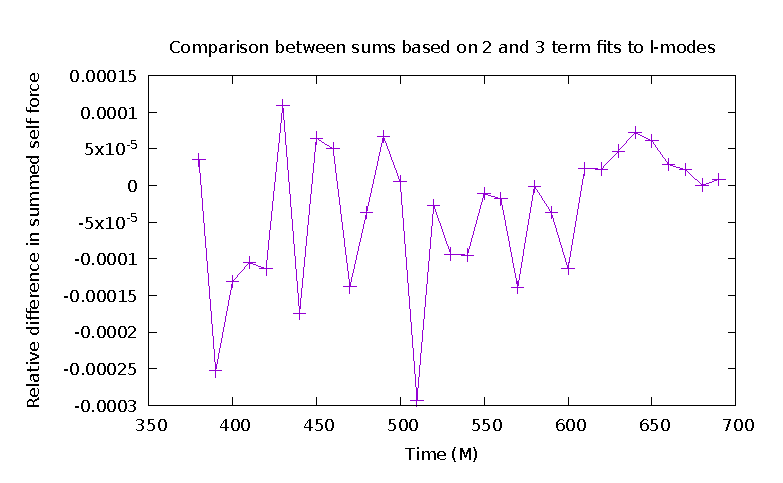
\includegraphics[width=\textwidth]{relativeError23termSelfForce}
      \caption{2 versus 3 terms}
    \end{subfigure}
  \caption{Relative errors in both of these effects appear to be at the $10^{-4}$ level.}
  \end{figure}
\end{frame}


\begin{frame}
  \frametitle{Smooth evolution of total radial self-force}
  \begin{figure}
    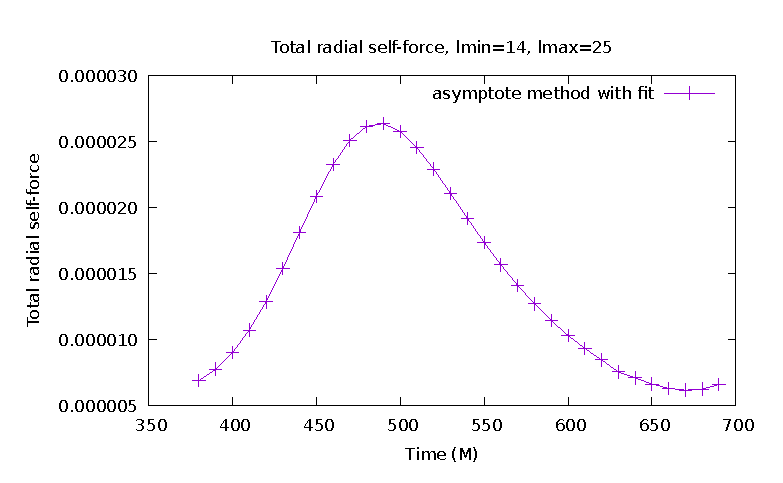
\includegraphics[width=0.9\textwidth]{totalselfforcevt2}
     \caption{Total radial self-force including sum to $l=\infty$ over time}
  \end{figure}
\end{frame}


\begin{frame}
  \frametitle{Error analysis conclusions}
  \begin{itemize}
  \item The relative error due to neglecting the first order Richardson extrapolation is $10^{-4}$. The best order at which to run is DG order 36. Limit dominated by roundoff error.
  \item The best $l_{min}=14$ and $l_{max}$=25. The relative error in these choice of values is $10^{-4}$.
  \item The relative error due to the number of terms used in the fit is $10^{-4}$.
  \item The error due to the use of weights in fitting is insignificant.
  \item These results are preliminary and need further investigation.    
  \end{itemize}
\end{frame}

\end{document}
